\documentclass[11pt,a4paper,oneside,openany]{report}

\usepackage{graphicx}
\usepackage{tabularx}
\usepackage{subfigure}
\usepackage{afterpage}
\usepackage{amsmath,amssymb}            
\usepackage{rotating}  
\usepackage{fancyhdr}  
\usepackage[scriptsize]{caption}
\usepackage{listings}
\hyphenation{a-gen-tiz-za-zio-ne}

\setlength{\paperwidth}{16cm}
\setlength{\paperheight}{24cm}
\setlength{\oddsidemargin} {2. cm}
\setlength{\evensidemargin} {2. cm}
\addtolength{\oddsidemargin} {-0.4 cm}
\addtolength{\evensidemargin} {-0.4 cm}
\linespread{1.1}

\usepackage[english]{babel}
\usepackage[latin1]{inputenc}
\renewcommand{\captionfont}{\normalfont \sffamily \itshape \small}

\pagestyle{empty}

\begin{document}


\thispagestyle{empty}
%\begin{titlepage}
\vspace*{-1.5cm} \bfseries{
\begin{center}
  \large
  POLITECNICO DI MILANO\\
  \normalsize
  Corso di Laurea Magistrale in Ingegneria Informatica\\
  Dipartimento di Elettronica e Informazione\\
  \begin{figure}[htbp]
    \begin{center}
      
\includegraphics[width=3.5cm]{./pictures/logopm}
% 
\psfig{file=./pictures/logopm.jpg,width=3.5cm}
    \end{center}
  \end{figure}
  \vspace*{0.3cm} \LARGE

  \textbf Fine-grained Autonomic Systems With Containers\\

  \vspace*{.75truecm} \large
  DEIB \\
  Dipartimento di Elettronica,   \\
  Informatica e Bioingegneria del Politecnico di Milano
\end{center}
\vspace*{3.0cm} \large
\begin{flushleft}


  Relatore: Prof. Luciano Baresi \\
  Correlatore: Dott. Giovanni Quattrocchi 

\end{flushleft}
\vspace*{1.0cm}
\begin{flushright}


  Tesina di Laurea di:\\ Dmitrii Stebliuk, matricola 823716 \\ 


\end{flushright}
\vspace*{0.5cm}
\begin{center}



  Academic Year 2015-2016
\end{center} \clearpage
}

\thispagestyle{empty} \normalfont \cleardoublepage
\vspace{17cm}

%\large
\begin{flushright}
\itshape{ Dedicated to my family and everybody who supports me through thesis and master degree period}
\end{flushright}
\thispagestyle{empty}  \cleardoublepage
\pagenumbering{Roman}
\newpage
\chapter*{Abstract}

\addcontentsline{toc}{chapter}{Abstract}
This paper presents the research on Autonomic Systems with different types of virtualization. It were investigated coarse-grained virtualization techniques like virtual machines or cloud instances, and light-weight fine-grained techniques like operating system-level virtualization (containers). The thesis scope is implementation demo case of Autonomic System using different virtualization elements and considering the advantages and disadvantages of using containers for building Autonomic Systems.
\thispagestyle{empty} \vspace*{.75truecm} \cleardoublepage
\chapter*{Acknowlegements}

\addcontentsline{toc}{chapter}{Acknowlegements}

I would like to thank Politecnico Di Milano professors of the courses I took for the dedication to their work and interesting, cutting-edge material they were teaching us.

\vspace{0.5cm}
\noindent Also I would like to thank my supervisor Giovanni Quattrocchi for guiding and supporting me all other my thesis production period.

\thispagestyle{empty}
\begin{center}
    \tableofcontents
\end{center}
\pagenumbering{arabic}
\pagestyle{plain}\renewcommand{\chaptermark}[1]{\markboth{\chaptername\ \thechapter.\ #1}{}} 
\renewcommand{\sectionmark}[1]{\markright{\thesection.\ #1}}         

\fancyhead[LO]{\bfseries\rightmark}     
\renewcommand{\headrulewidth}{0.3pt} 

\chapter{Introduction}
\label{introduction}
\thispagestyle{empty}

\noindent
Nowadays software can consist of many different parts that are running together. The functional and non functional requirements are subject to continuous changing and the service infrastructure should be capable to support these changes. A concrete example of automatic infrastructure management is Amazon's AutoScaling, which manage when and how an application's resources should be dynamically increase or decrease. This paper describes implementation of alternative solution that help to solve autoscaling problems.

\section{General idea}
\begin{sloppypar}This paper describes Autonomous Systems management using different types of virtualization: virtual machines and containers. This Autonomous System adaptation is based on the MAPE framework: "M" stands for monitoring, "A" for analysing, "P" for planning and "E" for execution. In other words the system is monitored, analysed and the adaptation plan is produced that is executed by some driver depending on what virtualization technique we choose.
\end{sloppypar}

\ifx La prima parte contiene una frase che spiega l'area generale dove si svolge il lavoro; una che spiega la sottoarea pi\`u specifica dove si svolge il lavoro e la terza, che dovrebbe cominciare con le seguenti parole ``lo scopo della tesi \`e \dots'', illustra l'obbiettivo del lavoro. Poi vi devono essere una o due frasi che contengano una breve spiegazione di cosa e come \`e stato fatto, delle attivit\`a sperimentali, dei risultati ottenuti con una valutazione e degli sviluppi futuri. La prima parte deve essere circa una facciata e mezza o due
\fi

\section{Autonomic system}
Autonomic system is self-adapting self-managing system with distributed resources, that can adapt to unpredictable changes while hiding intrinsic complexity to operators and users. 
IBM was on of the first companies who suggested this kind of systems and it has set forth eight conditions that define an autonomic system:
The system must
\begin{enumerate}
    \item know itself in terms of what resources it has access to, what its capabilities and limitations are and how and why it is connected to other systems.
    \item be able to automatically configure and reconfigure itself depending on the changing computing environment.
    \item be able to optimize its performance to ensure the most efficient computing process.
    \item be able to work around encountered problems by either repairing itself or routing functions away from the trouble.
    \item detect, identify and protect itself against various types of attacks to maintain overall system security and integrity.
    \item The system must be able to adapt to its environment as it changes, interacting with neighboring systems and establishing communication protocols.
    \item rely on open standards and cannot exist in a proprietary environment.
    \item anticipate the demand on its resources while keeping transparent to users.
\end{enumerate}

Even though the purpose and thus the behaviour of autonomic systems vary from system to system, every autonomic system should be able to exhibit a minimum set of properties to achieve its purpose:
\begin{enumerate}
    \item Automatic: This essentially means being able to self-control its internal functions and operations. As such, an autonomic system must be self-contained and able to start-up and operate without any manual intervention or external help. Again, the knowledge required to bootstrap the system (Know-how) must be inherent to the system.
    \item Adaptive: An autonomic system must be able to change its operation (i.e., its configuration, state and functions). This will allow the system to cope with temporal and spatial changes in its operational context either long term (environment customisation/optimisation) or short term (exceptional conditions such as malicious attacks, faults, etc.).
    \item Aware: An autonomic system must be able to monitor (sense) its operational context as well as its internal state in order to be able to assess if its current operation serves its purpose. Awareness will control adaptation of its operational behaviour in response to context or state changes.
\end{enumerate}

\section{MAPE The IBM Autonomic Framework}
The IBM Autonomic COmputing Initiative codified an external, feedback control approach in its Autonomic Monitor-Analyze-Plan-Execute (MAPE) Model. Figure 1 illustrates the MAPE loop, which distinguishes between the autonomic manager (embodied in the large rounded rectangle) and the managed element, which is either an entire system or a component within a larger system. The MAP loop highlights four essential apsects of self-adaptation:
\begin{enumerate}
    \item \textbf{Monitor}: The monitoring phase is concerned with extracting information - properties or states - out of the managed element. Mechanisms range from source-code instrumentation to non-intrusive communication interception.
    \item \textbf{Analyze}: is concerned with determining if something has one away in the system, usually because a system property exhibits a value outside of expected bounds, or has a degrading trend.
    \item \textbf{Plan}: is concerned with determining a course of action to adapt the managed element once a problem is detected.
    \item \textbf{Execute}: is concerned with carrying out a chosen course of action and effecting the changes in the system.
\end{enumerate}
 
\begin{figure}[h]
  \centering
    
\includegraphics[natwidth=264,natheight=198]{./pictures/mape}
    \caption{Fig. 1 The IBM Autonomic MAPE Reference model}
\end{figure}
  

\section{Cloud and coarse-grained virtualization}
Modern web applications more often are run in the cloud. By the cloud it is very often means that application is deployed not on real physical (bare-metal) machine, but on the virtual machine where virtual infrastructure can be configured on the cluster of machines. This approach has advantages to classic bare-metal one. First of all it is scalability: as machine is virtual we can do vertical scaling (allocate CPU cores or RAM) as we want, moreover if the cloud infrastructure works on the cluster, we can provide resources that one real machine just do not have. The second advantage is again scaling: we can easily create new virtual machines this is called horizontal scaling. And the last advantage is on-demand computing or pay-as-you-go, when you do not need to pay upfront, but only for the resources you use.

\begin{sloppypar}
Current implementation uses Amazon Elastic Cloud Computing as cloud provider. Also it is supported Vagrant. Vagrant is software that is higher-level wrapper around virtualization software such as VirtualBox, VMWare, KVM, Linux containers and Amazon EC2. Vagrant and Amazon EC2 drivers do not use vertical scaling features, but only the horizontal one: creating/deling new virtual machines. This scaling is considered as coarse-grained, because Amazone EC2 VM and VirtualBox VM takes quite long time to create and use heavy virtualization technologies: like full-virtualization, paravirtualization or hardware-assisted virtualization.
\end{sloppypar}

This is in the opposite to light-weight operation system-level virtualization based on Linux containers. Current implementation uses docker engine for managing containers. With containers vertical scaling (allocation CPU cores and RAM) and horizontal scaling (creating/ deleting new containers) is much faster than the same operation with full virtualization.

\section{Containers}
Container virtualization it is operating-system-level virtualization method where the kernel of an operating systems allows for multiple isolated user-space instances, instead of just one.
For current implementation we use docker implementation of container virtualization. It uses modern Linux features like LXC containers and cgroups for managing resources. 
Containers have some advantages comparing to classic full-virtualization: they have very low or zero overhead, because they are running without emulation and just send system signals to operation system kernel. Moreover containers are much more faster to create/delete as they do not need to start / stop operation system that can take significant amount of time. On the other hand containers are not considered as classic virtualization killers, that will take its place. Current approach is to use classic virtualization for clouds, and run container above classic virtual machines, so the containers virtualization is used above the classic one.

\begin{figure}[h]
  \centering
    
\includegraphics[width=335px,height=217px,natwidth=770,natheight=434]{./pictures/docker-vm-container}
    \caption{Fig. 2 Comparing VM to container}
\end{figure}

\section{Contribution}
The main contribution was implementing the "E" executor part of MAPE framework applied to autonomous system. Different implementation cases were researched with different virtualization techniques and implementations.
First of all executor accepts as the input the plan from the  "P" planner. It was considered two different implementations of executor: "monolithic" and "distributed". The difference between them is that the monolithic executor manages virtual machines on its own, it decides when it is required to create/delete virtual machine, the input plan goes to the main node, which orchestrates agent nodes (virtual machines) with docker containers. The distributed executor manages only containers on the virtual machines and the plan goes directly to the agent, so the executor does not need to estimate the number of virtual machines or try to solve allocation problem.

Also the executor considers different types of virtualization: coarse-grained one (full-virtualization, hardware-assisted or paravirtualization) and the operation system-level virtualization (containers). For coarse-grained virtualization it were implemented drivers for vagrant and amazon elastic compute cloud, that supports a lot of different virtualization types. For containers the driver for docker was implemented. 

Also for continuously changing environment it should be implemented some configuration adjustment. For example after scaling JBOSS application from using 1 CPU and 2gb RAM to 8 CPU and 16gb RAM, we want to run instead of 4 JBOSS threads, 32 threads. This requirement was implemented as "scale-hooks" which are run on each docker container creation/update. Also sometimes configuration adjustment should be more complex, taking the same example with JBOSS resources update, load balancing node needs to change weights or to add new nodes to its configuration. So load balancing node should wait for finishing of create/update operations on each JBOSS node and after that trigger its adjustment. This type of adjustment we call "tier-hooks" and for them should be specified dependency, for example load balance node depends on JBOSS tier. After each change of JBOSS tier, the tier-hooks are run for the nodes that depends on the changed tier.


\ifx {Breve descrizione del lavoro}
La seconda parte deve essere una esplosione della prima e deve quindi mostrare in maniera pi\`u esplicita l'area dove si svolge il lavoro, le fonti bibliografiche pi\`u importanti su cui si fonda il lavoro in maniera sintetica (una pagina) evidenziando i lavori in letteratura che presentano attinenza con il lavoro affrontato in modo da mostrare da dove e perch\'e \`e sorta la tematica di studio. Poi si mostrano esplicitamente le realizzazioni, le direttive future di ricerca, quali sono i problemi aperti e quali quelli affrontati e si ripete lo scopo della tesi. Questa parte deve essere piena (ma non grondante come la sezione due) di citazioni bibliografiche e deve essere lunga circa 4 facciate.
\fi

\section{Thesis structure}
The second part describes functional and non functional requirements for the executor module of the MAPE framework.
Also it describes solution design, considering initial problems, approaches, decisions made and architecture chosen.

The third part describes the technologies, algorithms and implementation details.

\ifx 
{Struttura della tesi}
La terza parte contiene la descrizione della struttura della tesi ed \`e organizzata nel modo seguente.
``La tesi \`e strutturata nel modo seguente.

Nella sezione due si mostra \dots

Nella sez. tre si illustra \dots

Nella sez. quattro si descrive \dots

Nelle conclusioni si riassumono gli scopi, le valutazioni di questi e le prospettive future \dots

Nell'appendice A si riporta \dots (Dopo ogni sezione o appendice ci vuole un punto).''

I titoli delle sezioni da 2 a M-1 sono indicativi, ma bisogna cercare di mantenere un significato equipollente nel caso si vogliano cambiare. Queste sezioni possono contenere eventuali sottosezioni.
\fi
\chapter{Requirements}
\label{requirements}
\section{Introduction}

The following requirements describe the system called \textbf{Executor}. The main goal of the \textbf{Executor} is to provide required infrastructure and resources to the controlled micro-services.
Under micro-service we understand some 1-tier or multi-tier application. We consider only 2 types of resources: CPU cores and available RAM. 

The required infrastructure and resources are provided by creating Virtual Machines and allocating containers on them. Each container is considered to store 1 tier of the application. If tier requires more resources than 1 VM has then this tier would be represented by more than 1 container on different VMs.

The input of the executor is the \textbf{topology} and the \textbf{plan}. 
The \textbf{topology} describes each application and its tiers:
static information which can be changed only by change topology request. The \textbf{plan} says how many resources is required for each tier. 

The plan can be of two different types: the \textbf{monolithic} one and the \textbf{distributed}. The \textbf{monolithic} plan means that it says just how many resources it needs for each tier and the \textbf{Executor} considering current \textbf{allocation} tries to decide how many VMs it needs to create / delete and how it should allocate containers on all VMs to satisfy all \textbf{plan} requirements. Current \textbf{allocation} it is information about currently used VMs and containers and tiers running on them.

The \textbf{distributed} plan takes VMs management on its own and specifies tiers resources demand for each VM separately. It says that on this VM, this tier needs this number of CPU cores and this number of available RAM.

Also continuously adjusted system requires some triggers to be run on the adjustment. The system requires two types of triggers: one that runs on each container after scaling (container create / update) and another that runs after some dependee tier (container) is scaled. We will call these triggers \textbf{hooks}. For example the first \textbf{scale hooks} are used when we need to adjust a number of threads considering how many resources container has. The second \textbf{tier hooks} are used by load balancer, which may be needs to change weights for tiers after dependee containers are changed. Also \textbf{tier hooks} can be used to provide information about dependee tiers: for example JBOSS tiers needs IP address of DB tier.

\section{Specific requirements}
This section contains all requirements for the Executor: functional, non-functional and constraints. Each requirement is described in the following sections:
\begin{table}[ht]
  \begin{tabular}{|p{3.5cm}|p{8cm}|}
  \hline
    \textbf{Requirement ID}  & \begin{sloppypar}Uniquely identifiers requirement \end{sloppypar}\\
  \hline
    \textbf{Title}  & \begin{sloppypar}Gives the requirement a symbolic name\end{sloppypar}\\
  \hline
    \textbf{Description}  & \begin{sloppypar}The definition of the requirement\end{sloppypar}\\
  \hline
    \textbf{Priority}  & \begin{sloppypar}Defines the order in which requirements should be implemented. Priorities are designated (highest to lowest) from 1 to 3. Requirements of priority 1 are mandatory; 2 represents features nice to have, and 3 represents optional features.
    \end{sloppypar}\\
  \hline
    \textbf{Risk}  & \begin{sloppypar}
Specifies the risk of not implementing the requirement. It shows how critical the requirement is to the system as a whole. The following risk levels are defined over the impact of not being implemented correctly.
    \begin{itemize}
        \item \textbf{Critical (C)} It will break the main functionality of the system. The system cannot be used if this requirement is not implemented.
        \item \textbf{High (H)} It will impact the main functionality of the system. Some function of the system could be inaccessible, but the system can be generally used.
        \item \textbf{Medium (M)} It will impact some system features, but not the main functionality. The system can still be used with some limitation.
        \item \textbf{Low (L)} The system can be used without limitation, but with some workarounds.
    \end{itemize} \end{sloppypar}\\
  \hline
  \end{tabular}
\end{table}
\clearpage
\subsection{Functional requirements}

\begin{table}[ht]
  \begin{tabular}{|p{3.5cm}|p{8cm}|}
  \hline
    \textbf{Requirement ID}  & FR-0 \\
  \hline
    \textbf{Title}  & \begin{sloppypar}The user should set topology of the system\end{sloppypar}\\
  \hline
    \textbf{Description}  & \begin{sloppypar}The topology includes:
      \begin{itemize}
        \item Infrastructure description
            \begin{itemize}
                \item Driver used (Vagrant, AWS)
                \item VM resources (CPU cores and RAM)
                \item VM image
                \item Credentials (Optional)
            \end{itemize}

        \item Max VMs value
        \item Application list
        \item Tiers list of each applications
        \item Scalability of the tier
        \item Docker image of the tier
        \item Scale hooks
        \item The tier dependencies list
        \item Tier hooks
      \end{itemize}
    \end{sloppypar}\\
  \hline
    \textbf{Priority}  & 1\\
  \hline
    \textbf{Risk}  & C \\
  \hline
  \end{tabular}
\end{table}

\begin{table}[ht]
  \begin{tabular}{|p{3.5cm}|p{8cm}|}
  \hline
    \textbf{Requirement ID}  & FR-1 \\
  \hline
    \textbf{Title}  & \begin{sloppypar}The user should emulate the monolithic plan execution\end{sloppypar}\\
  \hline
    \textbf{Description}  & \begin{sloppypar}The user should provide the monolithic plan to the system and get the result as list of actions executed: VMs created / deleted, containers created / deleted / updated, scale hooks run and tier hooks run \end{sloppypar}\\
  \hline
    \textbf{Priority}  & 2\\
  \hline
    \textbf{Risk}  & M \\
  \hline
  \end{tabular}
\end{table}

\begin{table}[ht]
  \begin{tabular}{|p{3.5cm}|p{8cm}|}
  \hline
    \textbf{Requirement ID}  & FR-2 \\
  \hline
    \textbf{Title}  & \begin{sloppypar}The user should execute the monolithic plan\end{sloppypar}\\
  \hline
    \textbf{Description}  & \begin{sloppypar}The plan should describe the required resources for all the tiers of the application.\end{sloppypar}\\
  \hline
    \textbf{Priority}  & 1\\
  \hline
    \textbf{Risk}  & C \\
  \hline
  \end{tabular}
\end{table}

\begin{table}[ht]
  \begin{tabular}{|p{3.5cm}|p{8cm}|}
  \hline
    \textbf{Requirement ID}  & FR-3 \\
  \hline
    \textbf{Title}  & \begin{sloppypar}The user should see the current allocation\end{sloppypar}\\
  \hline
    \textbf{Description}  & \begin{sloppypar}The system should show the created VMs with its IP addresses and tiers containers with allocated resources.\end{sloppypar}\\
  \hline
    \textbf{Priority}  & 1\\
  \hline
    \textbf{Risk}  & C \\
  \hline
  \end{tabular}
\end{table}

\iffalse
\begin{table}[ht]
  \begin{tabular}{|p{3.5cm}|p{8cm}|}
  \hline
    \textbf{Requirement ID}  & FR-00000 \\
  \hline
    \textbf{Title}  & \begin{sloppypar}TITLE \end{sloppypar}\\
  \hline
    \textbf{Description}  & \begin{sloppypar}DESCRIPTION\end{sloppypar}\\
  \hline
    \textbf{Priority}  & 1\\
  \hline
    \textbf{Risk}  & C \\
  \hline
  \end{tabular}
\end{table}
\fi
\chapter{Solution design}
\label {solutiondesign}

The executor contains of two parts: the main node and the agents. The agent runs on the created VMs, manages starting / updating / removing of the docker containers, executing of the distributed plan and provides information about current allocation and docker inspect output. The main node manages executing of the monolithic plan, and also provides current allocation and docker inspect output. The main node provides the allocation by sending requests to each known agent and aggregating answers.

\section{Problems}
\subsection{Bin packing problem}
  The monolithic approach given current allocation and the monolithic plan (resource demand for each tier) should do creation / deletion of VMs and allocation containers on them. This problem is similar to well-known Bin packing problem. A VM for us is a bin and a container is an object which we need to pack in the bin. The container has two dimensions: CPU cores and RAM, so this is 2D bin packing problem. The main difference to bin packing problem is that we have initial allocation (initial packing) and we should not only minimize number of bins used, but also number of movements required to reach the final allocation from the initial one.
  
  The linear optimisation problem was formulated to solve this 2d bin packing problem:
  
\begin{equation*}
\text{minimize } \displaystyle\sum\limits_{i \in I}^{}\sum\limits_{j \in J}^{} (w_{0ij} \alpha_{0ij} + w_{1ij} \alpha_{1ij}) + \sum\limits_{i \in I}^{} (w_{2i} \beta_{0i} + w_{3i} \beta_{1i})
\end{equation*}
\begin{equation*}
\begin{array}{ll@{}ll}
\text{subject to} & & &\\
\text{(1)}           & \displaystyle\sum\limits_{j \in J}^{} x_{ij} \leq m_{0i} \beta_{0i}  & & \forall i \in I\\
\text{(2)}           & \displaystyle\sum\limits_{j \in J}^{} y_{ij} \leq m_{1i} \beta_{0i} & & \forall i \in I\\
\text{(3)}           & \displaystyle  x_{ij} \leq m_{0i} \alpha_{ij} & & \forall i \in I, j \in J\\
\text{(4)}           & \displaystyle y_{ij} \leq m_{1i} \alpha_{ij} & & \forall i \in I, j \in J\\
\text{(5)}           & \displaystyle\sum\limits_{i \in I}^{} x_{ij} = d_{0j} & & \forall j \in J\\
\text{(6)}           & \displaystyle\sum\limits_{i \in I}^{} y_{ij} = d_{1j} & & \forall j \in J\\
\text{(7)}           & \displaystyle m_{1i} x_{ij} \geq y_{ij} & & \forall i \in I, j \in J\\
\text{(8)}           & \displaystyle m_{0i} y_{ij} \geq x_{ij} & & \forall i \in I, j \in J\\
\text{(9)}           & \displaystyle \alpha_{0ij} + \alpha_{1ij} = 1 & & \forall i \in I, j \in J\\
\text{(10)}          & \displaystyle \beta_{0i} + \beta_{1i} = 1 & & \forall i \in I\\
                     & \alpha_{0ij} \in \{0, 1\}  & & \forall i \in I, j \in J\\
                     & \alpha_{1ij} \in \{0, 1\}  & & \forall i \in I, j \in J\\
                     & \beta_{0i} \in \{0, 1\}  & & \forall i \in I\\
                     & \beta_{1i} \in \{0, 1\}  & & \forall i \in I\\
                     & x_{ij} \in \mathbb{Z}  & x_{ij} \geq 0 & \forall i \in I, j \in J\\
                     & y_{ij} \in \mathbb{Z}  & y_{ij} \geq 0 & \forall i \in I, j \in J\\
\end{array}
\end{equation*}
where \\
\indent $I$ is the set of VMs,\\
\indent $J$ is the set of Tiers,
\begin{sloppypar} $\alpha_{0ij}$ is "tier\_is\_used" binary variable that is true if we allocate container for tier[j] on VM[i],
\indent $\alpha_{1ij}$ is "tier\_is\_idle" binary variable that is true only if $\alpha_{0ij}$ is false, the equation (9) links them together,
\indent $\beta_{0i}$ is "vm\_is\_used" binary variable that is true if we allocate any container for any tier on VM[i],
\indent $\beta_{1i}$ is "vm\_is\_idle" binary variable that is true only if $\beta_{0i}$ is false, the equation (10) links them together,
\indent $x_{ij}$ is "cpu\_usage" variable: the number of CPU cores that tier[j] uses on VM[i],
\indent $y_{ij}$ is "mem\_usage" variable: "the number of RAM units (1 unit = 512Mb) that tier[j] uses on VM[i],
\indent (1) is CPU availability constraint and constraint for activation of "vm\_is\_used" variable, constant $m_{0i}$ is the number of CPU cores on VM[i] (maximum allowed value for $x_{ij}$),
\indent (2) is the same as (1), but for the RAM units, constant $m_{1i}$ is the number of RAM units on VM[i] (maximum allowed value for $y_{ij}$) 
\indent (3) and (4) are activation of $\alpha_{ij}$ constraints similar to (1) and (2). (3) is for CPU cores, (4) is for RAM units,
\indent (6) is the RAM units demand equation, where $d_{1j}$ is the RAM units demand from the plan for the tier[j],
\indent (5) is the same as (4), but for the CPU cores, $d_{0j}$ is the CPU cores demand from the plan for the tier[j],
\indent (7) says that if tier[j] uses some RAM on VM[i], then it must use some CPU cores,
\indent (8) is the same as constraint (7), but other way round: if tier[j] uses some CPU cores on VM[i], then it must use some RAM units.
\end{sloppypar}

This formulation of the problem requires us to know the number of VMs beforehand, which we do not know. So the upper bound number of VMs is calculated and provided to the ILP solver. VMs that are used in the initial allocation are already created, but there are also VMs that are empty and are only going to be created if there will be some container on it.

Considering the initial allocation is done by constants $w_{0ij}, w_{1ij}, w_{2i}, w_{3i}$.
Where $w_{0ij}$ is the constant for using tier[j] on VM[i], so knowing initial allocation we can set this constant to the cost of the container creation if there is no tier[j] on VM[i] in the initial allocation, and the cost of the container update if there is tier[j] on VM[i] in the initial allocation. Here is a pitfall that if in the initial allocation container was used on the VM, and we use it in the new allocation, we can not differentiate if the value of CPU cores and RAM units used has changed (we need to run container update command) or is not changed (we need do nothing).

The weight constant $w_{1ij}$ is the cost of removing container of the tier[j] from the VM[i], this weight should be 0 if the tier[j] was not on the VM[i] in the initial allocation.

The weight $w_{2i}$ is the cost of VM[i] creation. if VM[i] is already used in the initial allocation this constant is 0.

The weight $w_{3i}$ is the cost of using the VM[i]. This cost is 0, if 
the VM is not created yet, and it was not used in the initial allocation.

Considering NFR-2, the weights for actions should follow these rules: 
\begin{enumerate}
    \item container delete \textless{ } container update \textless{ } container create
    \item VM delete \textless{ } VM use \textless{ } VM create
    \item VM delete + container delete  + container create \textless{ } \\ VM use + container update
\end{enumerate}

 \begin{sloppypar} The rule number 3 is introduced, because it is possible a situation when for example we can remove some VM[p], this VM had in the initial allocation 1 container. The weight of vm\_usage=30, the weight of vm\_deletion=25, the weight of container\_update=10, the weight of container\_deletion=5, the weight of container\_create=15. So to continue to use this VM the objective function will have $vm\_usage + container\_update=30 + 10 = 40$, and to remove this container in the worst case we need to create container in another place: $vm\_deletion + container\_deletion + container\_create = 25 + 5 + 15 = 45$. So ILP minimizing the objective function will choose not to remove the VM[p], but keep it. This is against our requirement NFR-0 and we want to keep the minimum number of VMs possible. 
 \end{sloppypar}
 
 Also NFR-2 requires weight of "container use" be less than "container update", but I could not found the easy way to differentiate them in ILP. As we have initial allocation as constants, for example $c_{ij}$ is CPU cores used by container[j] on VM[i] and $m_{ij}$ is the same for RAM units. The new allocation in the ILP are variables $x_{ij}$ and $y_{ij}$ for CPU cores and RAM units accordingly. So to differentiate "container use" from "container update", we need either $x_{ij} + y_{ij} \neq c_{ij} + m_{ij}$ or $abs(x_{ij} + y_{ij} - c_{ij} - m_{ij}) > 0$ or some "if" constraint that all makes our ILP non linear. The effective workaround to solve this issue is considered out of scope of this paper.

\subsection{Scalability}
The tier can be scalable or not. The not scalable tier can have only 1 or 0 containers. If the tier is absent in the plan, it will have 0 containers, otherwise it will be 1, whilst the scalable tier can have any number of containers $\geq 0$ allocated on different VMs. In the ILP formulation not scalable containers are not considered, so the current workaround is too 

\subsection{Limitation of the ILP formulation}
This ILP formulation has some limitations:
\begin{enumerate}
    \item This formulation of the problem requires us to know the number of VMs beforehand, which we do not know. But we can make upper-bound estimation.
    \item This formulation does not differentiate between "container update" and "container use" (do nothing with container). 
    \item Weights should be chosen wisely to satisfy NFR-0.
    \item Bin packing problem is NP-hard
    \item We have 1 optimal solution and can not choose between several different solutions
\end{enumerate}

\subsection{Hooks}
Hooks are scripts that trigger on the tier / container scaling. The goal is to adjust the application's configuration after the allocation is changed.

We tried to extract and describe use cases of adjusting required:
\begin{enumerate}
    \item Jboss needs to adapt the number of threads considering the number of CPU allocated.
    \item LoadBalancer needs to be provided with the list of Jboss containers and resources allocated to adapt it weights.
    \item Jboss needs to be provided with the DB address on container creation / change.
\end{enumerate}

The adjustment 1 should be run for the container after it is created or updated. We call this adjustment "scale-hook" or "on\_node\_scale" hook. The script should be provided with 4 arguments: previous CPU cores allocated, previous RAM memory units allocated, and new CPU cores and RAM memory units allocated.

In the 2nd adjustment   the LoadBalancer tier depends on the Jboss tier. So the dependencies should be specified. Also the dependent node (LoadBalancer) should wait until all the containers of the dependee are processed (JBOSS). After that the adjustment script should be run on all the containers of the dependent node (LoadBalancer). We call this adjustment "tier-hook" or "on\_dependency\_scale" hook.

The 3d adjustment should be run only on the container start. To simpliy the first version of the application we decided not to implement this adjustment for the dependecy 1-to-n. Only for the dependencies n-to-1 and 1-to-1 after the dependee tier is processed, the ip of the dependee tier is provided to the dependent node on the creation (parameter "add-host"). 

This creates some limitations: the dependee container should be processed before dependent containers. For example, if the first plan will have only dependent containers, in the next plan it will be added dependee container, and in the last plan the dependence between them will be specified, then "add-host" feature will not be propagated and the dependee containers will not know about the dependant one.

Similar problem if we decided to remove the not-scalable tier from the plan, the dependee containers will have not valid "add-host" link and even if later we put the "not-scalable" tier back to the plan, it will have another IP address.

So considering these limitations we suggest one of the two workarounds.

The first is to manage the DB dependencies out of the topology and provide the IP address in the topology as "docker parameter".

The second is just use docker "add-host" feature as it. So if the dependent container is removed, or the dependency is added, the user should be aware that "add-host" will not be specified.

\subsection{Dependencies}
Considering the requirement FR-9 only 1-to-1, 1-to-n and n-to-1 dependencies are supported. The dependencies between scalable tiers are not supported. The dependencies are only used to manager tier-hooks and . 
The flow for container allocation and hooks execution should be:
\begin{enumerate}
    \item get tiers dependency graph (G)
    \item get set of Tiers without outgoing dependencies (T)
    \item run container create / update / delete for each tier in T
    \item run scale hooks if needed for each tier container in T
    \item run tier hooks if needed for each tier container in T
    \item remove T from G
    \item if G is not empty go to 2
\end{enumerate}

\section{Approaches}
Besides the ILP approach to solve container allocation problem discussed above it was also tried another approache: Constraint Satisfaction Problem.

\subsection{Constraint Satisfaction Problem}

CSP is defined as a triple \textless X, D, C\textgreater, where $X$ is a set of variables, $D$ is a set of the respective domains of values, $C$ is a set of constraints.

In our context we have 2 matrices of variables as $X$: \\
$x_{ij}$ is a matrix that specify how many CPU is used by Tier[j] on VM[i],\\
$y_{ij}$ is a matrix that specify how many RAM units are used by Tier[j] on VM[i].

The domain $D$ for us is all possible values of CPU cores and RAM units. For example if we have AWS t2.medium with 2 CPU cores and 8 RAM units, we have: \\
$d_{0ij}$ is $\{0, 1, 2\}$ for CPU cores,\\
$d_{1ij}$ is $\{0, 1, 2, 3, 4, 5, 6, 7, 8\}$ for RAM mem units.

For a set of constraints $C$ we should consider similar to ILP:
\begin{itemize}
    \item availability constraints on each VM for CPU cores and for RAM mem units
    \item demand constraint considering the plan
    \item 0 CPU cores with RAM \textgreater{} 0 or other way round
\end{itemize}

\subsection{Limitation of the CSP}
This CSP formulation has also some limitations:
\begin{enumerate}
    \item Comparing to ILP, changing domain to continuous values may cause problems.
    \item The solution of the CSP is a list of different solutions, that can differ only by a permutation. We can have a factorial number of different solutions which we need to look to found the optimal one considering the initial allocation.
    \item The problem is NP-Hard and the complexity growth is much faster than the ILP.
\end{enumerate}

The CSP formulation has one insuperable problem that it does not scale. If we have 10 Tiers, 10 VMs, and 16 CPU cores and 64 RAM mem units, the CSP solution does not complete in appropriate time.

\section{Architecture}

\begin{figure}[ht]
  \centering
    \includegraphics[width=350px,natwidth=688,natheight=617]{./pictures/architecture}
    \caption{Architecture}
\end{figure}

The architecture consists of two main components: Executor Main Node and Executor Agent. The main node accepts a monolithic plan, orchestrates agents 
and has a whole picture of VMs allocated. The agent node can accept a distributed plan to execute, can run / start / stop docker containers, provides the allocation information and output of docker inspect command.

These executor nodes are "Execute" part of the autonomous system MAPE framework. The Monitor component measures different metrics of applications that are
running in the containers on the Executor agents, and provide this information to the Analyze component. The Plan component together with the Analyze component produce a new plan (a resource demand for tiers) which is sent to Executor.

\clearpage
\subsection{Components}
\begin{figure}[ht]
  \centering
    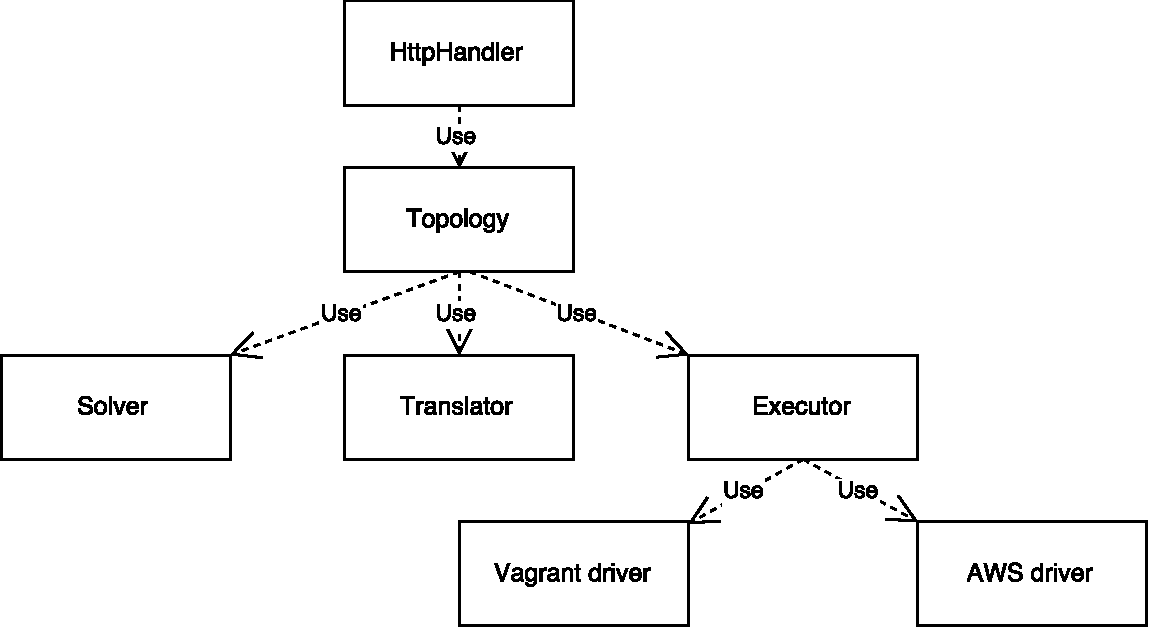
\includegraphics[width=350px,natwidth=553,natheight=303]{./pictures/main-classes}
    \caption{Executor main node classes}
\end{figure}

\begin{figure}[ht]
  \centering
    \includegraphics[natwidth=113,natheight=203]{./pictures/agent-classes}
    \caption{Executor agent node classes}
\end{figure}
\chapter{Implementation}
\label{implementation}

\section{Integer Linear Programming}
For prototype the ILP problem formulated in the section 3.1.1 was modeled and solved in AMPL language.

\begin{lstlisting}[caption=AMPL model]

set Tier; 
set VM;

param tier_used{Tier, VM}; 
param vm_used{VM};
param cpu_demand{Tier};
param mem_demand{Tier};
param cpu_max{VM};
param mem_max{VM};
param use_tier_weight{Tier, VM};
param use_vm_weight{VM};
param not_use_tier_weight{Tier, VM};
param not_use_vm_weight{VM};

var tier_usage{Tier, VM} >= 0 binary;
var vm_usage{VM} >= 0 binary;
var tier_idle{Tier, VM} >= 0 binary;
var vm_idle{VM} >= 0 binary;
var cpu{Tier, VM} >= 0 integer;
var mem{Tier, VM} >= 0 integer; 

minimize cost:
  sum{i in Tier, j in VM} 
    (use_tier_weight[i, j] * tier_usage[i, j] +
      not_use_tier_weight[i, j] * tier_idle[i, j]) + 
  sum{j in VM} (use_vm_weight[j] * vm_usage[j] + 
    not_use_vm_weight[j] * vm_idle[j]);

subject to CPU_availability{j in VM}:
  sum{i in Tier} 
    cpu[i, j] <= cpu_max[j] * vm_usage[j];

subject to RAM_availability{j in VM}:
  sum{i in Tier} mem[i, j] <= mem_max[j];

subject to CPU_demand{i in Tier}:
  sum{j in VM} cpu[i, j] = cpu_demand[i];

subject to RAM_demand{i in Tier}:
  sum{j in VM} mem[i, j] = mem_demand[i];

subject to CPU_activation{i in Tier, j in VM}:
  cpu_max[j] * tier_usage[i, j] >= cpu[i, j];

subject to RAM_activation{i in Tier, j in VM}:
  mem_max[j] * tier_usage[i, j] >= mem[i, j];

subject to CPU_RAM_activation{i in Tier, j in VM}:
  mem_max[j] * cpu[i, j] >= mem[i, j];

subject to RAM_CPU_activation{i in Tier, j in VM}:
  cpu_max[j] * mem[i, j] >= cpu[i, j];

subject to link_tier_idle{i in Tier, j in VM}:
  tier_idle[i, j] + tier_usage[i, j] = 1;

subject to link_vm_idle{j in VM}:
  vm_idle[j] + vm_usage[j] = 1;
\end{lstlisting}

In the executor we solve the problem using \textit{or-tools} and ILP solver by Google. The Solver component
accepts the current allocation, the topology and provides as output a new allocation. The new allocation is
the input of the Translator component which translates the new allocation to the list of actions to be run.
This list of actions is the input to the Executor component.

\section{API}
\subsection{Main Node}
\textbf{[GET] /api/allocation}
Returns the allocation JSON of known VMs. In reality, just make calls to VMs and groups answers.
\begin{lstlisting}[caption=Example GET allocation output,basicstyle=\tiny]
{
  "52.34.2.170": {
    "rubis_app_server":{  
      "cpuset": [0],
      "cpu_cores": 1,
      "mem_units": 2
    },
    "pwitter_app_server":{  
      "cpuset": [1],
      "cpu_cores": 1,
      "mem_units": 3
    }
  }
}
\end{lstlisting}

\vspace{5mm}
\textbf{[GET] /api/inspect}
Returns the inspect output JSON for known VMs. In reality, just make calls to VMs and groups answers.
\begin{lstlisting}[caption=Example GET inspect output,basicstyle=\tiny]
{
  "52.34.2.170": {  
    "rubis_app_server":{  
     "MemUnits": 2,
      "CpusetCpus": "0",
      "Memory":1073741824
    },
    "pwitter_app_server": {  
      "MemUnits": 3,
      "CpusetCpus": "1",
      "Memory": 1610612736
    }
  } 
}
\end{lstlisting}

\vspace{5mm}
\noindent\textbf{[GET] /api/topology} \\
Returns JSON with the current topology.
\begin{lstlisting}[caption=Example topology,basicstyle=\tiny]
{
  "infrastructure": {
    "cloud_driver": {
      "name": "aws-ec2",
      "autoscaling_group_name": "monolithic-ex-8cpu",
      "credentials": "/usr/me/utils/aws.properties"
    },
    "max_vms": 10,
    "hooks_git_repo": "https://github.com/n43jl/hooks.git"
  },
  "apps": [{
    "name": "rubis",
    "tiers": {
      "loadbalancer": {
        "name": "Front Load Balancer",
        "max_node": 1,
        "docker_image": "haproxy",
        "depends_on": ["app_server"],
        "on_dependency_scale": "reload_server_pool.sh",
        "max_rt": 0.1
      },
      "app_server": {
        "name": "Application Logic Tier",
        "docker_image": "polimi/rubis-jboss",
        "depends_on": ["db"],
        "on_node_scale": "jboss_hook.sh",
        "on_dependency_scale": "reload_connections.sh",
        "ports": ["80:8080"],
         "entrypoint_params": "-w 3 -k eventlet"
      },
      "db": {
        "name": "Data Tier",
        "max_node": 1,
        "docker_image": "mysql",
        "on_node_scale": "mysql_hook.sh",
        "max_rt": 0.2,
        "ports": ["3306:3306"]
      }
    }
  },{
    "name": "pwitter",
    "tiers": {
      "app_server": {
        "name": "Application Logic Tier",
        "docker_image": "pwitter-web",
        "ports": ["8080:5000"],
        "entrypoint_params": " /opt/jboss-4.2.2.GA/bin/run.sh --host=0.0.0.0 
        --bootdir=/opt/rubis/rubis-cvs-2008-02-25/Servlets_Hibernate -c default"
      },
      "db": {
        "name": "Data Tier",
        "max_node": 1,
        "docker_image": "mysql",
        "on_node_scale": "mysql_hook.sh",
        "max_rt": 0.2,
        "ports": ["3307:3306"]
      }
    }
  }],
} 
\end{lstlisting}

\vspace{5mm}
\noindent\textbf{[PUT] /api/topology} \\
Set the topology. The payload is the same as the example output of the [GET] /api/topology method.

\vspace{5mm}
\noindent\textbf{[PUT] /api/translate} \\
Returns JSON with the actions list required to execute provided in the payload plan.
\begin{lstlisting}[caption=Example of the input payload,basicstyle=\tiny]
{
  "rubis": {
    "app_server": {
      "cpu_cores": 1,
      "mem_units": 3
    }
  },
  "pwitter": {
    "app_server": {
      "cpu_cores": 1,
      "mem_units": 4  
    }
  }
}
\end{lstlisting}
\begin{lstlisting}[caption=Example of the output,basicstyle=\tiny]
{  
  "actions":[  
    "update container \"rubis_app_server\" 
     on the vm "52.34.2.170" set cpu_cores=1 and mem_units=3",
    "update container \"pwitter_app_server\" 
     on the vm "52.34.2.170" set cpu_cores=1 and mem_units=4"
  ]
}
\end{lstlisting}



\subsection{Agent}
\textbf{[GET] /api/allocation} \\
Returns JSON with the current allocation of the containers on the VM. The difference with the "inspect" command is that
"inspect" is the output of "docker inspect" command, while the "allocation" is taken from the app runtime state. e.g. We
create using the API some container "Jboss". Both the "allocation" and "inspect" will return 1 container. After that we 
stop / start our Executor Agent Node. The "allocation" will be empty, but the "inspect" will return 1 container.
\begin{lstlisting}[caption=Example GET allocation output,basicstyle=\tiny]
{  
  "rubis_app_server":{  
    "cpu_cores": 1,
    "mem_units": 2
  },
  "pwitter_app_server":{
    "cpu_cores": 1,
    "mem_units": 3
  }
}
\end{lstlisting}

\vspace{5mm}
\noindent\textbf{[GET] /api/inspect} \\
Returns JSON with the current docker containers running on the VM.
\begin{lstlisting}[caption=Example GET inspect output,basicstyle=\tiny]
{  
  "rubis_app_server":{  
    "MemUnits": 2,
    "CpusetCpus": "0",
    "Memory":1073741824
  },
  "pwitter_app_server": {  
    "MemUnits": 3,
    "CpusetCpus": "1",
    "Memory": 1610612736
  }
}
\end{lstlisting}

\vspace{5mm}
\noindent\textbf{[GET] /api/topology} \\
The output is the same as for the main node.

\vspace{5mm}
\noindent\textbf{[PUT] /api/topology} \\
The input and the output is the same as for the main node.

\vspace{5mm}
\noindent\textbf{[PUT] /api/translate} \\
Returns JSON with the actions list required to execute provided in the payload plan.
\begin{lstlisting}[caption=Example of the input payload,basicstyle=\tiny]
{
  "rubis": {
    "app_server": {
      "cpu_cores": 1,
      "mem_units": 3
    }
  },
  "pwitter": {
    "app_server": {
      "cpu_cores": 1,
      "mem_units": 4  
    }
  }
}
\end{lstlisting}
\begin{lstlisting}[caption=Example of the output,basicstyle=\tiny]
{  
  "actions":[  
    "update container \"rubis_app_server\" set cpu_cores=1 and mem_units=3",
    "update container \"pwitter_app_server\" set cpu_cores=1 and mem_units=4"
  ]
}
\end{lstlisting}

\vspace{5mm}
\noindent\textbf{[PUT] /api/topology} \\
Set the topology. The payload is the same as the example output of the [GET] /api/topology method.

\vspace{5mm}
\noindent\textbf{[PUT] /api/execute} \\
Returns JSON with the actions list required to execute provided in the payload plan.
\begin{lstlisting}[caption=Example of the input payload,basicstyle=\tiny]
{
  "rubis": {
    "app_server": {
      "cpu_cores": 1,
      "mem_units": 3
    }
  },
  "pwitter": {
    "app_server": {
      "cpu_cores": 1,
      "mem_units": 4  
    }
  }
}
\end{lstlisting}

\vspace{5mm}
\noindent\textbf{[PUT] /api/run/tier\_hooks} \\
Returns JSON with the actions list required to execute provided in the payload plan.
\begin{lstlisting}[caption=Example of the input payload,basicstyle=\tiny]
[
  {
    "app": "rubis",
    "dependent": "app_server",
    "depends_on": ["db"],
    "allocation": "..."
  }
]
\end{lstlisting}

\vspace{5mm}
\noindent\textbf{[PUT] /api/docker/run} \\
Runs the docker container specified in the payload.
\begin{lstlisting}[caption=Example of the input payload,basicstyle=\tiny]
{
  "name":"pwitter_app_server",
  "cpu_cores": 2,
  "mem_units": 3
}
\end{lstlisting}

\noindent\textbf{[PUT] /api/docker/remove} \\
Removes the docker container specified in the payload.
\begin{lstlisting}[caption=Example of the input payload,basicstyle=\tiny]
{  
  "name":"pwitter_app_server"
}
\end{lstlisting}

\noindent\textbf{[PUT] /api/docker/update} \\
Returns JSON with the actions list required to execute provided in the payload plan.
\begin{lstlisting}[caption=Example of the input payload,basicstyle=\tiny]
{  
  "name":"pwitter_app_server",
  "cpu_cores": 1,
  "mem_units": 2
}
\end{lstlisting}


\section{Topology}
There are restrictions for the topology:
\begin{enumerate}
    \item Ports are specified in the form (host VM port : guest container port). All hosts ports specified for all tiers should be unique, even for different applications.
    \item The script name specified in the "on\_node\_scale" should be located in the repository specified in "hooks\_git\_repo" in the folder "scale\_hooks".
    \item The script name specified in the "on\_dependency\_scale" should be located in the repository specified in "hooks\_git\_repo" in the folder "tier\_hooks".
    \item The max\_node=1 means that the tier is not scalable. It will not be moved from one VM to another and it must have the resources demand less than it is available on one VM.
    \item For tiers with the max\_node \textgreater{} 1 is allowed to have dependencies only to tiers with max\_node=1 (n-to-1). n-to-n dependencies are not allowed.
    \item Dependencies between tiers from different applications are not allowed.
    \item Circular dependencies are not allowed
\end{enumerate}

Also tier names should be unique inside the app, and the app name should be unique too. Any tiers of any apps can be on the same VM, so uniqueness of the container name is imposed by using as container name the compound name: "{APP\_NAME}\_{TIER\_NAME}".

\section{Hooks}
To adjust to the new allocation they should be provided with input parameters.

The "on\_node\_scale" hook requires as the input parameter the previous resources and the new. So there are 4 input parameters: previous CPU cores, previous memory units, new CPU cores and new memory units.

The "on\_dependency\_scale" hook requires the IP address of the dependee tier and new allocation resources. So the input parameters are: the dependee tier name, the dependent tier name and stringified allocation JSON.

\section{Algorithms}
\subsection{Processing list of actions}
\begin{figure}[ht]
  \centering
    \includegraphics[height=550px,natwidth=219,natheight=635]{./pictures/algorithm1}
    \caption{Processing list of actions }
\end{figure}
The algorithm figure 4.1 describes the workflow in processing the list of actions for containers and processing hooks. First of all the tiers that depends on other tiers should be processed only after the dependee. To support this we build the dependency graph and process tiers without dependencies first and after remove them from the graph.

The second is the order of processing a tier. We should first create containers, after we can do update and only after that we can do remove. This is done to have more resources than it required for the tiers, otherwise the monitor component may detect that applications needs more resources.

All the hooks (scale-hooks and tier-hooks) are run only they are specified for this tier.


\subsection{Processing plan}
\begin{figure}[ht]
  \centering
    \includegraphics[height=550px,natwidth=202,natheight=714]{./pictures/algorithm2}
    \caption{Processing the plan }
\end{figure}
Processing the plan is specified in the figure 4.2.
While processing the plan, the plan "app -\textgreater{} tier -\textgreater{} demand" is flatten to the form "app\_tier -\textgreater{} demand". 
If the demand is not equal to allocation than the ILP formulation is built and solved. As the result we get the new resource allocation considering VMs and containers with resources on them.
The procedure "process list of actions" is described in the figure 4.1.

\clearpage
\subsection{Translation}

The goal of the translation is to express the new allocation as the list of actions considering the current allocation. The set of possible actions considering we the container with the name "app\_tier" and the VM with the IP "127.0.0.1":
\begin{itemize}
    \item Create VM '127.0.0.1'
    \item Delete VM '127.0.0.1'
    \item Create container 'app\_tier' on the VM '127.0.0.1' with cpu=2 and mem=2.5gb
    \item \begin{sloppypar}Update container 'app\_tier' on the VM '127.0.0.1' set cpu=1 and mem=1gb\end{sloppypar}
    \item Run scale\_hooks for the container 'app\_tier' on the VM '127.0.0.1'
    \item Delete container 'app\_tier" on the VM '127.0.0.1'
    \item Run tier\_hooks for the container 'app\_tier' on the VM '127.0.0.1'
\end{itemize}

The algorithm for this translation is:
\begin{lstlisting}[caption=Translation algorithm]
FOR ALL vm IN current_allocation:
  IF vm IN new_allocation:
    FOR ALL container IN current_allocation[vm]:
      IF not container IN new_allocation[vm]:
        push_delete_container_action
  ELSE:
    push_delete_vm_action
FOR ALL vm IN new_allocation:
  IF vm IN current_allocation:
    FOR ALL container IN new_allocation[vm]:
      IF container IN old_allocation[vm]:
        push_update_container_action_if_needed
        push_run_scale_hooks_if_needed
      ELSE:
        push_create_container_action
        push_run_scale_hooks_if_needed
  ELSE:
    push_create_vm_action
    FOR ALL container IN new_allocation[vm]:
      push_create_container_action
      push_run_scale_hooks_if_needed
\end{lstlisting}

Scale-hooks run after each container update / create. Tier-hooks can be handled only considering the dependency graph. The executor adds tier-hooks to the list of actions.

\section{Monolithic vs Hierarchical approach}

\begin{figure}[ht]
  \centering
    \includegraphics[width=350px,natwidth=684,natheight=687]{./pictures/arch-hierachical}
    \caption{Hierarchical Executor}
\end{figure}

The current approach with solving a plan using ILP formulation we call the "monolithic" approach. Considering that all the implementation is run in the MAPE framework environment for the monolithic approach we have a global planner. Having a global planner has some drawbacks, as the control loop timeout should be at least the time required to run the plan (considering the VM creation take a long time for our test it was approximately 150s).

To go around large control loop timeouts we decided that MAPE components can be hierarchically spread among all the VMs and containers. So instead of having the one global planner, we want to have planner for each container. This we call the hierarchical approach.

In the hierarchical approach for each container there is the planner which produce the plan for its own container. To handle the VM constraints in CPU cores and memory, the VM has another planner that consolidates all containers plan and resolves this constraints. In the future work we are thinking to have the CPU requirement in the plan as the float number, this simplifies the constraint resolving considering each plan.

After plans are built for each VM, it hierarchically goes to the root planner and the root planer provides the plan to the master node executor. The master node executor accepts the plan, but it do not run it until the plans from each VM have arrived. This is because of the tier-hooks. To support tier-hooks we need to execute actions in the particular order (calculated by the dependency-graph), so we can not run some actions, until we know all the actions we need to run.

\section{Drivers}
There were implemented several drivers for managing virtual / cloud infrastructure: Vagrant, AWS, Docker.

As vagrant is an interface (a facade) to large list of different virtualization providers and AWS also supports very large list of vitalization (even Docker containers). This 3 cases covers a lot of different virtualization techniques.

\subsection{Vagrant driver}
Vagrant was used mostly during the implementation stage of the work to test everything locally without paying for Amazon AWS infrastructure.

The image for Vagrant is based on the "ubuntu/trusty64" image with docker and "Ecoware executor agent" installed.

All ports that are required for tiers should be preconfigured in the Vagrantfile. The application "Ecoware executor agent" uses the port 8000, which should be also preconfigured in the Vagrant file. The Vagrant configuration files can be found in the repository.

Vagrant is something like an interface or a facade to list of the virtualization providers. As providers Vagrant supports:
\begin{itemize}
    \item VirtualBox
    \item VMware
    \item Hyper-V
    \item Docker
    \item You can develop your own plugin for custom provider
\end{itemize}
Using Vagrant helps to abstract from different providers and make it easy to change providers without changing our driver.

To manage Vagrant our driver uses the python module \textit{subprocess} to call OS commands like \textit{vagrant up}

\subsection{AWS driver}
For implementing AWS driver it were tested 3 different ways to communicate with AWS:
\begin{enumerate}
    \item HTTP REST calls
    \item AWS management console
    \item Python AWS SDK boto3
\end{enumerate}
As all the code for the paper was written in the python, it was decided that using boto3 is the simplest and cleanest way.

In current implementation it was easier to use the AWS Auto Scaling Groups to create VMs. So creating VMs now is based on the "desired capacity" method for Auto Scaling Groups in AWS. So the workflow for creating VMs now is:
\begin{enumerate}
    \item Get required VM number from ILP solution (n).
    \item Set desired capacity for the Auto Scaling Group to n.
    \item Poll number of instances in the Auto Scaling Group until it equals to n.
    \item Poll the status of all instances of the Auto Scaling Group to be the "in service".
    \item Get IP addresses of all VMs.
    \item Analyse the previous allocation, the new allocation and separate existed machines with the new.
    \item Set the topology to the new VMs, on error sleep 10s and repeat.
\end{enumerate}

The "polling" in this context means to make the request to the AWS and if the result is not satisfactory, sleep 10s, and repeat the request again.

Creating the VM takes approximately 150s.

For the deletion of the VM we can not just set the desired capacity to the smaller number, because we need to delete some particular machine, but not any one from all machines. To remove particular machine we just do 2 actions:
\begin{enumerate} 
    \item Detach the instance from the autoscaling group.
    \item Terminate the instance
\end{enumerate}

The AWS infrastructure supports different virtualization techniques:
\begin{itemize}
    \item HVM
    \item PV
    \item Docker containers
\end{itemize}
HVM stands for Hardware-Assisted Virtualization. 
PV stands for Paravirtualization.
In spite of the fact that these virtualization techniques are different and have its own advantages and disadvantages, AWS helps us to abstract from this and use its unified API.

To configure AWS for using with AWS driver it is required to do some steps:
\begin{description}
    \item [AMI.] The AMI should contain the \textit{Ecoware Executor Agent} and docker installed. The \textit{Ecoware Executor Agent} and docker engine should be in the autostart. All the containers images that will be used for different tiers should be pulled in the docker. Also all the containers should be removed to not have the name collision.
    \item [Security Group.] Security Group should be configured considering all the ports that containers want to listen to and the \textit{Ecoware Executor Agent} default port 8000.
    \item [Launch Configuration.] Launch Configuration should be created considering the AMI we want to use, the security group, and the AWS instance type.
    \item [Auto Scaling Group.] Auto Scaling Group should be created using the Launch Configuration with the initial instance number equals to 0.
\end{description}

\subsection{Docker driver}
Besides the fact that both Vagrant and AWS support Docker containers as under layer virtualization technique (or the provider), we use docker without any facade or interface, but directly. This helps to simplify and separate the separation between fine-grained and coarse-grained virtualization.

Docker is managed as the Vagrant using OS calls with the python module \textit{subprocess}.

\begin{sloppypar}The command to run have this structure (example of the run action):\end{sloppypar}

\begin{lstlisting}[caption=Docker run template,basicstyle=\small]
docker run -itd {PORTS} {HOSTS} --cpuset-cpus={CPUS} 
  -m={MEM}m --name={NAME} -v=/ecoware:/ecoware {IMAGE} 
  {ENTRY_PARAMS}
\end{lstlisting}

\begin{lstlisting}[caption=Docker run example,basicstyle=\small]
docker run -itd -p 8080:5000 --add-host="db:172.31.31.123"
  --cpuset-cpus=0,1 -m=512m --name=rubis_app_server 
  -v=/ecoware:/ecoware pwitter-web -w 3 -k eventlet
\end{lstlisting}

\textit{-it} option means to allocate a tty for the container process (to run it interactively).\\
\textit{-d} option means to run container in the \textit{detached} mode (background mode).\\
The variable \textit{\{PORTS\}} is built considering ports specified in the topology.\\
The variable \textit{\{HOSTS\}} is built if the tier has dependency n-to-1 or 1-to-1.\\
Variables \textit{\{CPUS\}} and \textit{\{MEM\}} is resources demand from the plan.\\
The variable \textit{\{NAME\}} is built from the topology like\\ "\{APP\_NAME\}\_\{TIER\_NAME\}".\\
\textit{-v} option means to add a data volume. The format is host\_dir:guest\_dir. The name of the directory is hardcoded, this is directory where the git repository with hooks is pulled.\\
The variable \textit{\{IMAGE\}} is taken from the topology.\\
The variable \textit{\{ENTRY\_PARAMS\}} is the entry point params also taken from the topology.


\section{Unit testing}
Some of the algorithms can be easily tested with unit-testing.

For example, the ILP algorithm is quite weight sensitive and tuning the weights can break some logic. Moreover there are many different ways how the system can satisfy the new plan and sometimes it is not clear and obvious which way is more optimal. So for the ILP solver it was written a list of the tests.

The input for the test is 3 json files: "plan.json", "result.json" and "allocation.json". So the iLP solver is tested that given the current allocation and the plan, it produces the new allocation equals to specified in the "result.json".

Any arguable ILP solution can be inspected in details and added to the tests.

Also algorithms like "building the dependency graph", "translation from allocation to actions" are tested too.

\clearpage
\section{UML}
\begin{figure}[ht]
  \centering
    \includegraphics[width=350px,natwidth=633,natheight=482]{./pictures/implementation-main}
    \caption{Class diagram for the executor on the Main Node}
\end{figure}

\begin{figure}[ht]
  \centering
    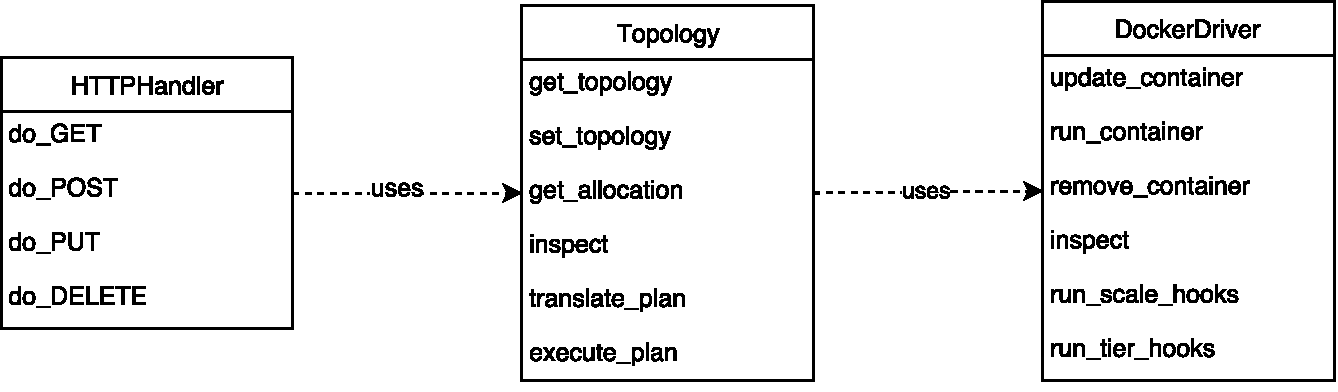
\includegraphics[width=350px,natwidth=643,natheight=190]{./pictures/implementation-agent}
    \caption{Class diagram for the executor on the Agent Node}
\end{figure}

\begin{figure}[ht]
  \centering
    \includegraphics[height=450px,natwidth=433,natheight=593]{./pictures/sequence}
    \caption{Sequence diagram}
\end{figure}

\clearpage
\section{Examples}
\subsection{The monolithic executor}
For example we have initially empty system without running VMs and containers. The topology of our applications is the same as in the listing 4.4. The executor is running locally on the port 8000: http://localhost:8000/. The autoscaling group "monolithic\_ex\_8cpu " is configured and it uses VMs with 8 CPU cores and 32gb of RAM (64 RAM units).

As the HTTP client we can consider the unix tool "curl". 

First we set the topology

\texttt{curl -X PUT -d @topology.json \$endpoint}\\
where "topology.json" file contains the same json as in the listing 4.4 and \$endpoint is
\texttt{http://localhost:8000/api/topology}

We can check the new topology opening in any browser \\ \texttt{http://localhost:8000/api/topology}.

For example now we want to start only the rubis application, giving 4 CPU cores and 4gb of RAM to "app\_server" and 1 CPU core and 4gb of RAM to the "db" tier.

For this example the payload.json" should be:

\begin{lstlisting}[caption=payload.json,basicstyle=\tiny]
{
  "rubis": {
    "app_server": {
      "cpu_cores": 4,
      "mem_units": 8
    },
    "db": {
      "cpu_cores": 1,
      "mem_units": 8
    }
  }
}
\end{lstlisting}

First, we can check which actions would be run for this plan by calling endpoint for translation. This call will not run these actions.

\texttt{curl -X PUT -d @payload.json \$endpoint}\\
the \$endpoint is \texttt{http://localhost:8000/api/translate}

After that we can execute the plan by calling the execute endpoint:

\texttt{curl -X PUT -d @payload.json \$endpoint}\\
where \$endpoint is \texttt{http://localhost:8000/api/execute}

We can check new allocation by calling these endpoints from the browser: \texttt{http://localhost:8000/api/allocation} and \\ \texttt{http://localhost:8000/api/inspect}.

After the planner decides to change the allocation of the containers it should just send to /execute/ endpoint the new payload with the new resources demand.
\chapter{Conclusion and future work}
\label{conclusion}

\section{Conclusion}
In this work it was implemented the Executor component for the autonomic system based with the adaption based on the MAPE framework. It were considered different virtualization types: coarse-grained the classic one (virtual machines) and the fine-grained container virtualization. During the implementing and experiments we can see advantages of container virtualization: using the fine-grained adaptation capabilities can greatly improve performance when autoscaling cloud-based web-application.

Modern cloud micro services and multitier architectures can benefit from using the autoscaling techniques, providing the decrease in the computational resource consuming, while showing high performance at the same time. The decreasing in the resource consumption it is not only sustainable approach to the environment, but also the reduction of the expenses considering the pay-as-you-go services like AWS.


\section{Future work}
As it is said in the conclusion part the adaptation using containers can greatly improve the performance of the autoscaling. As the evaluation part was not the part of this paper, the evaluation and the proof should be done as the future work.

Also as the future work it is considered the support of other infrastructure or cloud engines: Google App Engine or Microsoft Azure Cloud

Also the future work comprises the integration of feature adaptation by extending the adaptation hook mechanism, an extension of the planner to make it work hierarchically with respect to the controlled resources, and even finer-grained solution to control the CPUs cores allocated to a container, and further evaluation on more case studies of different kinds.

\cleardoublepage
\addcontentsline{toc}{chapter}{Bibliography}
\bibliographystyle{plain}
\bibliography{bibl_tesi}
\begin{thebibliography}{9}

\bibitem{mape}
Mieso Denko, Laurence Tianruo Yang, Yan Zhang.
\textit{Autonomic Computing and Networking.}
Springer Science \& Business Media, Jun 12, 2009.

\bibitem{monitor}
L. Baresi and S. Guinea.
\textit{Event-Based Multi-level
Service Monitoring.}
In Proceedings of the 20th
International Conference on Web Services, ICWS, pages 83\-90, 2013.

\bibitem{planner}
F. Seracini, M. Menarini, I. Krueger, L. Baresi,
S. Guinea, and G. Quattrocchi.
\textit{A Comprehensive
Resource Management Solution for Web-based
Systems.}
 In Proceedings of the 11th International
Conference on Autonomic Computing, ICAC - to
appear, 2014.

\bibitem{executor}
L. Baresi,
S. Guinea, and G. Quattrocchi.
\textit{Distributed Coordinated Adaptation
of Cloud-based Applications.}
Politecnico di Milano
Dipartimento di Elettronica, Informazione e Bioingegneria.

\bibitem{planner-new}
L. Baresi, S. Guinea, A. Leva, and G. Quattrocchi
\textit{A Discrete-Time Feedback Controller
for Containerized Cloud Applications}
Politecnico di Milano
Dipartimento di Elettronica, Informazione e Bioingegneria.

\bibitem{aws-autoscaling}
Amazon EC2 Autoscaling.\\
https://aws.amazon.com/autoscaling/.

\bibitem{aws-containers}
Amazon EC2 Container Service (ECS).\\
https://aws.amazon.com/ecs/.

\bibitem{docker}
Docker. \\
https://docker.com.

\bibitem{vagrant}
Vagrant.  \\
https://www.vagrantup.com.

\bibitem{cloud-computing}
M. Armbrust, A. Fox, R. Griffith, A. D. Joseph,
R. Katz, A. Konwinski, G. Lee, D. Patterson,
A. Rabkin, I. Stoica, and M. Zaharia.
\textit{A view of cloud
computing.}
Commun. ACM, 53(4):50-58, Apr. 2010.

\bibitem{self-adaptive}
H. Kienle, M. Litoiu, H. Müller, M. Pezzè, and
M. Shaw. Engineering self-adaptive systems through
feedback loops.
\textit{In Software engineering for
self-adaptive systems.}
Pages 48-70. Springer, 2009.

\bibitem{adaptation}
A. Gandhi, P. Dube, A. Karve, A. Kochut, and
L. Zhang.
\textit{Adaptive, model-driven autoscaling for
cloud applications.}
In 11th International Conference
on Autonomic Computing (ICAC 14), pages 57-64,
Philadelphia, PA, June 2014. USENIX Association.

\bibitem{asdfsadfasdfasdf}
Y. Hu, J. Wong, G. Iszlai, and M. Litoiu.
\textit{Resource
provisioning for cloud computing. In Proceedings of
the 2009 Conference of the Center for Advanced
Studies on Collaborative Research.}
Pages 101-111.
IBM Corp., 2009.

\iffalse
\bibitem{asdfasfasfasfasdfasf}
Amazonsafasdfsafasfdasdf \\
asfdsadfasfsadfsa

\bibitem{asdfsadfasdfasdf}
asdfasfasfasdfasdf
\textit{asdfasdfasdfasdf}
asdfasdfasdfasdfasdfasd

\bibitem{latexcompanion} 
Michel Goossens, Frank Mittelbach, and Alexander Samarin. 
\textit{The \LaTeX\ Companion}. 
Addison-Wesley, Reading, Massachusetts, 1993.
 
\bibitem{einstein} 
Albert Einstein. 
\textit{Zur Elektrodynamik bewegter K{\"o}rper}. (German) 
[\textit{On the electrodynamics of moving bodies}]. 
Annalen der Physik, 322(10):891 921, 1905.
 
\bibitem{knuthwebsite} 
Knuth: Computers and Typesetting,
\\\texttt{http://www-cs-faculty.stanford.edu/\~{}uno/abcde.html}
\fi


\end{thebibliography}


%\nocite{*}

\appendix

\pagestyle{fancy} 
\fancyfoot{}                                               
\renewcommand{\chaptermark}[1]{\markboth{\appendixname\ \thechapter.\ #1}{}} 
\renewcommand{\sectionmark}[1]{\markright{\thesection.\ #1}}         

\fancyhead[LO]{\bfseries\rightmark}     
\renewcommand{\headrulewidth}{0.3pt} 

\end{document}